% =====================================================================
%  Village Pond Planning System -- Final Technical Report
%  Compile:  tectonic main.tex        (or: xelatex main.tex, twice)
% =====================================================================
\documentclass[11pt,a4paper]{article}

% ---------- Fonts & layout (XeLaTeX / Tectonic) ----------------------
\usepackage{fontspec}
\usepackage{unicode-math}
\setmainfont{texgyrepagella}[Extension=.otf,UprightFont=*-regular,BoldFont=*-bold,
  ItalicFont=*-italic,BoldItalicFont=*-bolditalic]
\setsansfont{texgyreheros}[Extension=.otf,UprightFont=*-regular,BoldFont=*-bold,
  ItalicFont=*-italic,BoldItalicFont=*-bolditalic,Scale=MatchLowercase]
\setmonofont{lmmonolt10-regular.otf}[BoldFont=lmmonolt10-bold.otf,Scale=MatchLowercase]
\setmathfont{texgyrepagella-math.otf}
\usepackage[a4paper,margin=2.3cm,headheight=14pt]{geometry}
\usepackage{microtype}
\linespread{1.08}

% ---------- Packages -------------------------------------------------
\usepackage{xcolor}
\usepackage{graphicx}
\usepackage{booktabs,tabularx,multirow,longtable,array}
\usepackage{amsmath}
\usepackage{siunitx}
\sisetup{group-separator={,},group-minimum-digits=4,group-digits=integer,detect-all}
\usepackage[font=small,labelfont={bf,sf},format=hang]{caption}
\usepackage{subcaption}
\usepackage{enumitem}
\setlist{itemsep=2pt,topsep=4pt}
\usepackage{float}
\usepackage{fancyhdr}
\usepackage{titlesec}
\usepackage{tcolorbox}
\tcbuselibrary{skins,breakable}
\usepackage{listings}
\usepackage{algorithm}
\usepackage{algpseudocode}
\usepackage{tikz}
\usetikzlibrary{arrows.meta,positioning,shapes.geometric,shapes.multipart,fit,backgrounds,calc,shadows}
\usepackage[colorlinks=true,linkcolor=accent,citecolor=accent,urlcolor=accent]{hyperref}
\urlstyle{same}

% ---------- Colours --------------------------------------------------
\definecolor{accent}{HTML}{1C6FD1}
\definecolor{deep}{HTML}{12304F}
\definecolor{ink2}{HTML}{4A5666}
\definecolor{soft}{HTML}{E6F0FB}
\definecolor{good}{HTML}{1E7A4C}
\definecolor{warnc}{HTML}{8A5A00}
\definecolor{pond}{HTML}{FF3D71}
\definecolor{water}{HTML}{4A90D9}
\definecolor{soil}{HTML}{8A6D3B}

% ---------- Headings -------------------------------------------------
\titleformat{\section}{\sffamily\Large\bfseries\color{deep}}{\thesection}{0.8em}{}[\vspace{-2pt}{\color{accent}\titlerule[0.8pt]}]
\titleformat{\subsection}{\sffamily\large\bfseries\color{deep}}{\thesubsection}{0.7em}{}
\titleformat{\subsubsection}{\sffamily\normalsize\bfseries\color{ink2}}{\thesubsubsection}{0.6em}{}
\titlespacing*{\section}{0pt}{16pt}{8pt}

\pagestyle{fancy}
\fancyhf{}
\fancyhead[L]{\sffamily\small\color{ink2}Village Pond Planning System}
\fancyhead[R]{\sffamily\small\color{ink2}Technical Report}
\fancyfoot[C]{\sffamily\small\thepage}
\renewcommand{\headrulewidth}{0.4pt}

% ---------- Boxes ----------------------------------------------------
\newtcolorbox{keybox}[1][]{enhanced,breakable,colback=soft,colframe=accent,boxrule=0.6pt,arc=2pt,
  left=6pt,right=6pt,top=4pt,bottom=4pt,fonttitle=\sffamily\bfseries\small,title={#1}}
\newtcolorbox{notebox}[1][]{enhanced,breakable,colback=warnc!6,colframe=warnc!70,boxrule=0.6pt,arc=2pt,
  left=6pt,right=6pt,top=4pt,bottom=4pt,fonttitle=\sffamily\bfseries\small,title={#1}}

% ---------- Code -----------------------------------------------------
\lstset{basicstyle=\ttfamily\footnotesize,breaklines=true,frame=single,rulecolor=\color{black!20},
  backgroundcolor=\color{black!3},keywordstyle=\color{accent}\bfseries,commentstyle=\color{good},
  stringstyle=\color{warnc},columns=fullflexible,xleftmargin=4pt,xrightmargin=4pt,showstringspaces=false}

\newcommand{\code}[1]{\texttt{\small #1}}
\newcommand{\mcube}{\si{\cubic\metre}}
\newcolumntype{Y}{>{\raggedright\arraybackslash}X}

% =====================================================================
\begin{document}

% ---------------------------- Title page -----------------------------
\begin{titlepage}
\begin{tikzpicture}[remember picture,overlay]
  \fill[deep] (current page.north west) rectangle ([yshift=-8.2cm]current page.north east);
  \fill[accent] ([yshift=-8.2cm]current page.north west) rectangle ([yshift=-8.45cm]current page.north east);
  % stylised contours
  \begin{scope}[shift={([xshift=-4.2cm,yshift=-4.3cm]current page.north east)}]
    \foreach \r/\o in {0.6/0.9,1.1/0.7,1.6/0.55,2.1/0.4,2.6/0.28,3.1/0.18}
      \draw[white,opacity=\o,line width=0.7pt] plot[smooth cycle,tension=0.8]
        coordinates {(0,\r) (0.9*\r,0.5*\r) (1.1*\r,-0.3*\r) (0.3*\r,-\r) (-0.8*\r,-0.6*\r) (-\r,0.3*\r)};
    \fill[pond] (0.05,-0.05) circle (0.18);
    \draw[white,line width=1pt] (0.05,-0.05) circle (0.18);
  \end{scope}
\end{tikzpicture}

\vspace*{0.4cm}
{\color{white}\sffamily
{\small TECHNICAL REPORT \quad\textbullet\quad ASSIGNMENT 1}\\[0.9cm]
{\fontsize{27}{32}\selectfont\bfseries Village Pond\\[4pt] Planning System}\\[0.5cm]
{\large A geospatial decision-support web application for\\ siting and sizing rainwater-harvesting ponds}\par}

\vspace{4.2cm}
{\sffamily\large
\begin{tabular}{@{}l@{\hspace{1.2em}}l}
\textcolor{ink2}{Author}        & \textbf{Amandeeip Kammari} \\[3pt]
\textcolor{ink2}{Roll number}   & \textbf{12341060} \\[3pt]
\textcolor{ink2}{Date}          & September 2026 \\[3pt]
\textcolor{ink2}{Source code}   & \url{https://github.com/<your-username>/village-pond-planner} \\[3pt]
\textcolor{ink2}{Live system}   & \url{https://<your-app>.onrender.com}
\end{tabular}}

\vfill
\begin{tcolorbox}[colback=soft,colframe=accent,boxrule=0.6pt,arc=2pt]
\sffamily\small
\textbf{In one sentence.} Given only a village name, the system reconstructs the terrain,
maps land that is free for excavation, delineates catchments, retrieves twenty years of
satellite-gauge rainfall, simulates daily runoff and returns a ranked shortlist of pond sites
with engineering dimensions --- in about 40 seconds on first run and 3 seconds thereafter,
using only free public data.
\end{tcolorbox}
\end{titlepage}

% ---------------------------- Abstract --------------------------------
\pagenumbering{roman}
\section*{Abstract}
\addcontentsline{toc}{section}{Abstract}
Village ponds are among the most cost-effective rainwater-harvesting structures in rural India,
but choosing \emph{where} to dig one --- on land that is actually available, on a drainage line
that actually receives water, at a size the catchment can actually fill --- normally requires a
field survey and a hydrologist. This report presents a complete web application that automates
this preliminary planning from open data. A digital elevation model is assembled from global
terrain tiles (or interpolated from an uploaded KML contour map); surface flow is routed with
Priority-Flood depression filling and the D8 algorithm; land availability is inferred by an
OpenCV classifier on high-resolution satellite imagery combined with OpenStreetMap exclusions
and optional government land parcels; candidate sites are scored on flow accumulation, slope,
concavity and land suitability and then ranked so that each has an independent catchment;
twenty years of daily CHIRPS rainfall drive an antecedent-moisture-adjusted SCS Curve Number
runoff model; and a rectangular excavated pond is dimensioned to half of the 75\,\%-dependable
annual runoff, subject to land and depth constraints. Results are delivered through a FastAPI
back end and an accessible Leaflet front end with map overlays, charts, history and exports.

The system was validated component by component. Twenty-three unit tests check every formula
against hand calculations and an analytic catchment reproduced cell for cell. Against IMD
1991--2020 station normals, the chosen rainfall source (CHIRPS) has a mean absolute error of
\textbf{8.9\,\%}, compared with 26.1\,\% for NASA POWER, which overestimated Pune by 92\,\%;
this finding changed the system's default data source. The land-cover classifier reached
\textbf{92\,\% overall accuracy} ($\kappa=0.85$) on 100 blind-labelled cells from four
contrasting landscapes. A sensitivity analysis shows runoff has an elasticity of about three
with respect to rainfall, identifying rainfall as the dominant uncertainty in pond sizing. For
Hiware Bazar (Maharashtra), the system recommends five ponds with a combined storage of
\SI{121155}{\cubic\metre}, the best being a
\SI{141}{m}$\times$\SI{94}{m}$\times$\SI{3}{m} pond storing \SI{36856}{\cubic\metre} from a
\SI{138}{ha} catchment.

\vspace{6pt}
\noindent\textbf{Keywords:} rainwater harvesting; GIS; DEM hydrology; D8; SCS Curve Number;
CHIRPS; OpenCV; land-cover classification; FastAPI; Leaflet.

\clearpage
\tableofcontents
\clearpage
\listoffigures
\listoftables
\clearpage
\pagenumbering{arabic}

% =====================================================================
\section{Introduction}
% =====================================================================
\subsection{Problem}
Much of India's net sown area is rain-fed, and most of its rainfall arrives in the four months
of the south-west monsoon. Small surface storages --- farm ponds, village tanks,
\emph{Amrit Sarovars} --- capture this water for irrigation, livestock and groundwater recharge.
National programmes such as MGNREGA and Mission Amrit Sarovar fund thousands of such ponds a
year~\cite{amritsarovar}, but the quality of each investment depends on three decisions taken
early and often informally:
\begin{enumerate}
  \item \textbf{Where?} The pond must sit on a drainage line so that runoff reaches it, on
        gentle ground so that excavation is stable, and on land the village is actually allowed
        to dig --- normally gram-panchayat or government land.
  \item \textbf{How much water will arrive?} This depends on the catchment area, its land
        cover and soils, and the rainfall regime --- including dry years.
  \item \textbf{How big?} A pond much larger than its dependable inflow rarely fills; one much
        smaller wastes the catchment. Depth trades off evaporation losses against excavation
        cost and safety.
\end{enumerate}

\subsection{Objective and scope}
The objective, as set by the assignment, is a complete web application that analyses terrain
and rainfall to recommend suitable pond locations, estimates catchment area, rainfall
accumulation, pond depth and storage capacity, and presents the results on an interactive map.
The system is a \emph{pre-feasibility} tool: it narrows a village of several square kilometres
down to a handful of defensible candidate sites, each with quantified inflow and dimensions,
which an engineer can then verify in the field.

\subsection{Contributions}
\begin{itemize}
  \item An end-to-end pipeline that runs from a place name to ranked, dimensioned pond sites using
        only free public data and no GIS server software (Sections~\ref{sec:design}--\ref{sec:method}).
  \item A land-availability model fusing OpenCV image classification, OpenStreetMap features and
        user-drawn government parcels (Section~\ref{sec:land}).
  \item A candidate-ranking algorithm that guarantees hydrologically independent alternatives
        (Algorithm~\ref{alg:rank}).
  \item A daily, antecedent-moisture-aware SCS-CN runoff model and a constraint-driven pond
        design procedure (Sections~\ref{sec:runoff}--\ref{sec:pond}).
  \item A quantitative validation of every data source and algorithm, which led to replacing
        the initial rainfall dataset (Section~\ref{sec:validation}).
\end{itemize}

% =====================================================================
\section{Requirements}
% =====================================================================
\subsection{Functional requirements and traceability}
Table~\ref{tab:trace} maps each requirement in the brief to the modules, API fields and user
interface elements that satisfy it.

\begin{table}[H]
\centering\small
\caption{Requirement traceability matrix.}
\label{tab:trace}
\begin{tabularx}{\textwidth}{@{}p{0.4cm}>{\raggedright\arraybackslash}p{3.2cm}YY@{}}
\toprule
\# & Requirement & Implementation & Evidence in output \\
\midrule
1 & Satellite imagery for a selected village & Nominatim geocoding (\code{geocode.py}); Esri World Imagery basemap with place labels & Village search box; satellite map \\
2 & Visualise contour maps & OpenCV contour extraction from the DEM, or uploaded KML contours (\code{layers.py}); hillshaded relief & \code{layers.contours}, relief overlay \\
3 & Identify available land & OpenCV classification + OSM exclusions + parcels + slope (\code{landcover.py}) & \code{land}, \code{layers.suitable\_land} \\
4 & Catchment area & Priority-Flood, D8, reverse traversal, boundary tracing (\code{hydrology.py}) & \code{catchment}, boundary GeoJSON \\
5 & Historical rainfall via public APIs & CHIRPS (ClimateSERV), Open-Meteo, NASA POWER (\code{rainfall.py}) & \code{rainfall}: annual and monthly statistics \\
6 & Runoff volume & Daily SCS-CN with AMC adjustment; rational check (\code{runoff.py}) & \code{runoff} \\
7 & Pond depth and storage & Frustum design under land/depth constraints (\code{design.py}) & \code{pond\_design}, cross-section \\
8 & Overlay all results & Leaflet layers, charts, candidate table, exports (\code{static/}) & Map, sidebar, JSON/GeoJSON \\
\bottomrule
\end{tabularx}
\end{table}

\subsection{Non-functional requirements}
\begin{description}[style=nextline,leftmargin=1.2em]
  \item[Generality] No coordinate, village or result may be hard-coded; every output must derive
        from the input location or file.
  \item[Cost] Only free, key-less public data services may be required.
  \item[Performance] A full analysis should complete within about a minute on first run and in
        seconds when cached.
  \item[Robustness] The failure of any single external service must degrade the result, not
        abort it, and the degradation must be reported to the user.
  \item[Transparency] Every number must be traceable to its data source and method; the API
        returns the methods, parameters and timings used.
  \item[Accessibility] The front end must be usable by keyboard and screen reader and meet WCAG
        AA contrast.
\end{description}

% =====================================================================
\section{System design}\label{sec:design}
% =====================================================================
\subsection{High-level architecture}
The system is a three-tier web application (Figure~\ref{fig:arch}): a static single-page
front end, a stateless FastAPI application server containing all analysis logic, and a
persistence tier consisting of an SQLite database and an on-disk tile cache. External data
services are accessed only from the server, which lets it set proper User-Agent headers, cache
responses and keep API usage within fair-use limits.

\begin{figure}[H]
\centering
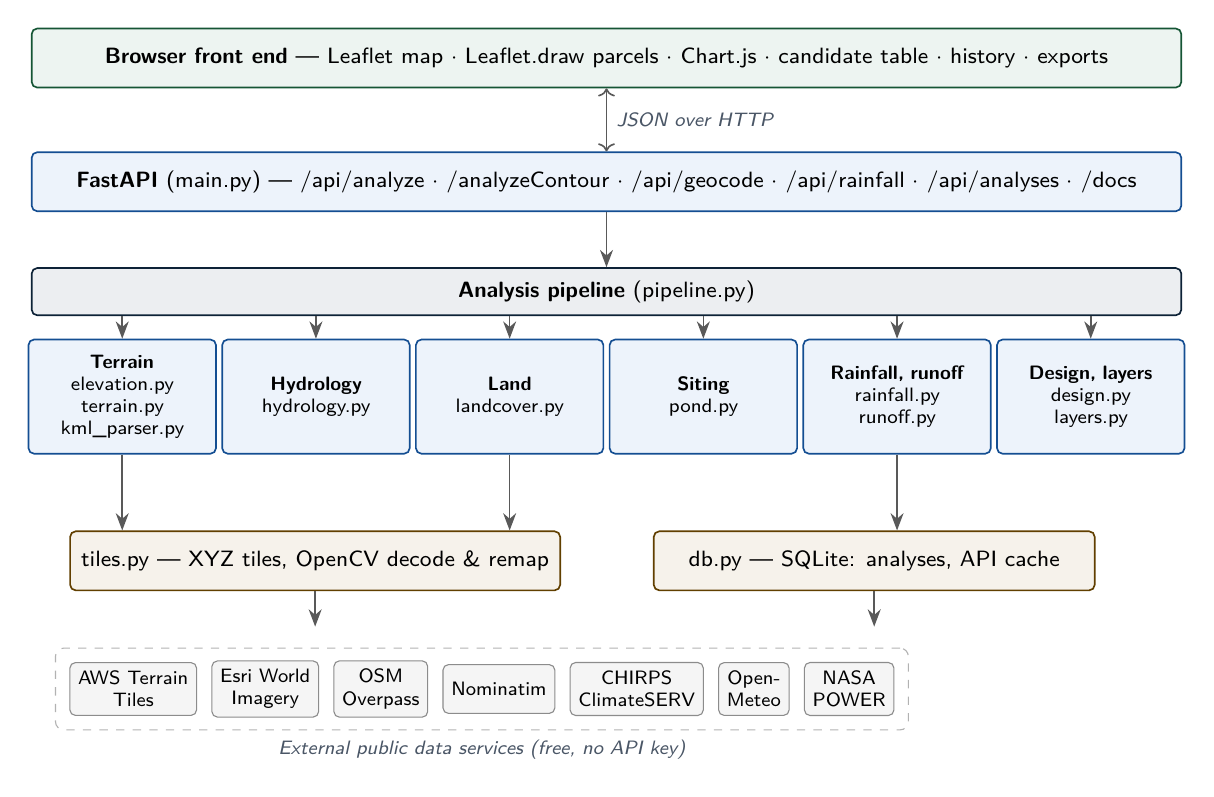
\begin{tikzpicture}[
  font=\sffamily\footnotesize,
  box/.style={draw=#1!70!black,fill=#1!8,rounded corners=2pt,minimum height=0.75cm,align=center,inner sep=4pt,line width=0.6pt},
  box/.default=accent,
  ext/.style={draw=black!45,fill=black!4,rounded corners=2pt,minimum height=0.62cm,align=center,inner sep=3pt,font=\sffamily\scriptsize},
  arr/.style={-{Stealth[length=2.2mm]},line width=0.6pt,color=black!65},
  lbl/.style={font=\sffamily\scriptsize\itshape,color=ink2}]
% Front end
\node[box=good,minimum width=14.6cm] (fe) at (0,0) {\textbf{Browser front end} --- Leaflet map $\cdot$ Leaflet.draw parcels $\cdot$ Chart.js $\cdot$ candidate table $\cdot$ history $\cdot$ exports};
% API
\node[box,minimum width=14.6cm,below=0.8cm of fe] (api) {\textbf{FastAPI} (main.py) --- /api/analyze $\cdot$ /analyzeContour $\cdot$ /api/geocode $\cdot$ /api/rainfall $\cdot$ /api/analyses $\cdot$ /docs};
\draw[arr,<->] (fe) -- node[right,lbl]{JSON over HTTP} (api);
% pipeline
\node[box=deep,minimum width=14.6cm,minimum height=0.6cm,below=0.7cm of api] (pipe) {\textbf{Analysis pipeline} (pipeline.py)};
\draw[arr] (api) -- (pipe);
% modules
\def\y{-4.3}
\tikzset{mod/.style={box,minimum width=2.3cm,text width=2.1cm,minimum height=1.45cm,font=\sffamily\scriptsize}}
\node[mod] (terr) at (-6.15,\y) {\textbf{Terrain}\\elevation.py\\terrain.py\\kml\_parser.py};
\node[mod] (hyd)  at (-3.69,\y) {\textbf{Hydrology}\\hydrology.py};
\node[mod] (land) at (-1.23,\y) {\textbf{Land}\\landcover.py};
\node[mod] (site) at (1.23,\y) {\textbf{Siting}\\pond.py};
\node[mod] (rain) at (3.69,\y) {\textbf{Rainfall, runoff}\\rainfall.py\\runoff.py};
\node[mod] (des)  at (6.15,\y) {\textbf{Design, layers}\\design.py\\layers.py};
\foreach \m in {terr,hyd,land,site,rain,des} \draw[arr] (pipe.south -| \m.north) -- (\m.north);
% infra
\node[box=warnc,minimum width=5.9cm,anchor=north] (tiles) at (-3.7,-6.0) {tiles.py --- XYZ tiles, OpenCV decode \& remap};
\node[box=warnc,minimum width=5.6cm,anchor=north] (db) at (3.4,-6.0) {db.py --- SQLite: analyses, API cache};
\draw[arr] (terr.south) -- (terr.south |- tiles.north);
\draw[arr] (land.south) -- (land.south |- tiles.north);
\draw[arr] (rain.south) -- (rain.south |- db.north);
% external
\node[ext,below=0.9cm of tiles.south west,anchor=north west] (e1) {AWS Terrain\\Tiles};
\node[ext,right=0.18cm of e1] (e2) {Esri World\\Imagery};
\node[ext,right=0.18cm of e2] (e3) {OSM\\Overpass};
\node[ext,right=0.18cm of e3] (e4) {Nominatim};
\node[ext,right=0.18cm of e4] (e5) {CHIRPS\\ClimateSERV};
\node[ext,right=0.18cm of e5] (e6) {Open-\\Meteo};
\node[ext,right=0.18cm of e6] (e7) {NASA\\POWER};
\begin{scope}[on background layer]
  \node[draw=black!30,dashed,rounded corners=3pt,fit=(e1)(e7),inner sep=5pt,label={[lbl]below:External public data services (free, no API key)}] {};
\end{scope}
\draw[arr] (tiles.south) -- ++(0,-0.45);
\draw[arr] (db.south) -- ++(0,-0.45);
\end{tikzpicture}
\caption{High-level architecture. Arrows show the direction of calls. Only the server talks to
external services; all responses are cached.}
\label{fig:arch}
\end{figure}

\subsection{Analysis data flow}
Figure~\ref{fig:flow} shows the processing stages of one analysis. The two input paths ---
village location or uploaded contour map --- converge on a common in-memory DEM, after which
the pipeline is identical. This separation is deliberate: every downstream algorithm depends
only on a regular elevation grid and a projection, so new terrain sources (GeoTIFF, drone
surveys) can be added without touching the hydrology.

\begin{figure}[H]
\centering
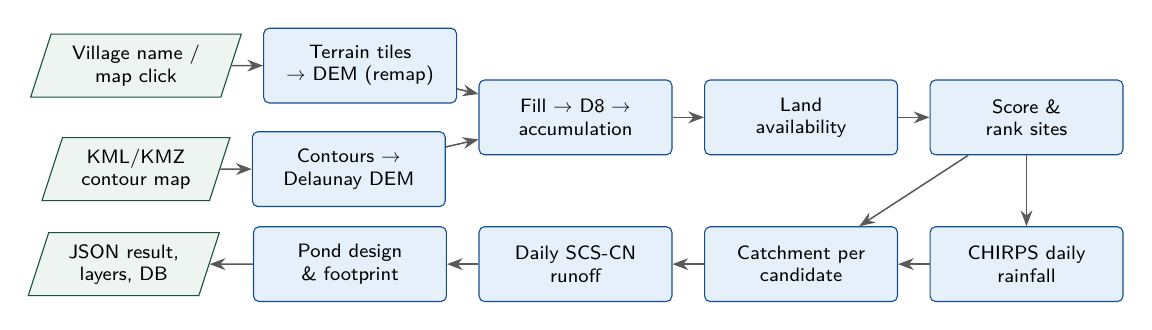
\begin{tikzpicture}[
  font=\sffamily\scriptsize,node distance=0.32cm and 0.4cm,
  st/.style={draw=accent!70!black,fill=soft,rounded corners=2pt,align=center,minimum width=2.45cm,minimum height=0.95cm,inner sep=2pt},
  io/.style={draw=good!70!black,fill=good!8,trapezium,trapezium left angle=72,trapezium right angle=108,align=center,minimum height=0.8cm,inner sep=2pt},
  arr/.style={-{Stealth[length=2mm]},line width=0.55pt,color=black!65}]
\node[io] (in1) {Village name /\\map click};
\node[io,below=0.5cm of in1] (in2) {KML/KMZ\\contour map};
\node[st,right=of in1] (dem1) {Terrain tiles\\$\rightarrow$ DEM (remap)};
\node[st,right=of in2] (dem2) {Contours $\rightarrow$\\Delaunay DEM};
\node[st,right=1.9cm of $(in1)!0.5!(in2)$,xshift=2.45cm] (hyd) {Fill $\rightarrow$ D8 $\rightarrow$\\accumulation};
\node[st,right=of hyd] (land) {Land\\availability};
\node[st,right=of land] (rank) {Score \&\\rank sites};
\node[st,below=0.9cm of rank] (rain) {CHIRPS daily\\rainfall};
\node[st,left=of rain] (catch) {Catchment per\\candidate};
\node[st,left=of catch] (run) {Daily SCS-CN\\runoff};
\node[st,left=of run] (des) {Pond design\\\& footprint};
\node[io,left=0.55cm of des] (out) {JSON result,\\layers, DB};
\draw[arr] (in1) -- (dem1); \draw[arr] (in2) -- (dem2);
\draw[arr] (dem1) -- (hyd); \draw[arr] (dem2) -- (hyd);
\draw[arr] (hyd) -- (land); \draw[arr] (land) -- (rank);
\draw[arr] (rank) -- (catch); \draw[arr] (rank) -- (rain);
\draw[arr] (rain) -- (catch);
\draw[arr] (catch) -- (run); \draw[arr] (run) -- (des); \draw[arr] (des) -- (out);
\end{tikzpicture}
\caption{Processing stages of one analysis. Rainfall is fetched once (at the top site) and
shared by all candidates, since they lie within the same few kilometres.}
\label{fig:flow}
\end{figure}

\subsection{Request sequence}
A village analysis is a single synchronous \code{POST /api/analyze} request. Within it, the
slow rainfall download (CHIRPS, two ten-year chunks in parallel) is overlapped with the
evapotranspiration download from a second service (Figure~\ref{fig:seq}). On a repeat request
for the same area every external call is served from the tile cache or the \code{api\_cache}
table.

\begin{figure}[H]
\centering
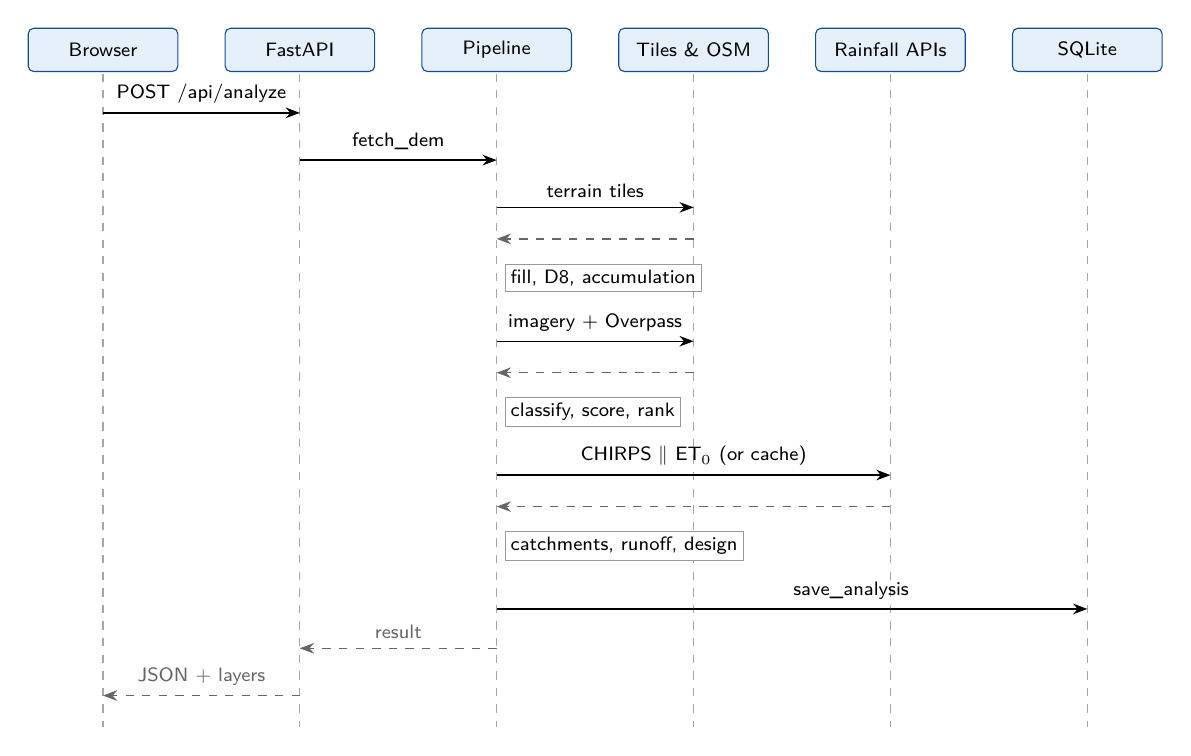
\begin{tikzpicture}[font=\sffamily\scriptsize,
  life/.style={draw=black!35,dashed},
  msg/.style={-{Stealth[length=1.8mm]},line width=0.5pt},
  ret/.style={-{Stealth[length=1.8mm]},dashed,line width=0.5pt,color=black!60},
  hd/.style={draw=accent!70!black,fill=soft,rounded corners=2pt,minimum width=1.9cm,minimum height=0.55cm,align=center}]
\foreach \x/\n/\t in {0/U/Browser,2.5/A/FastAPI,5/P/Pipeline,7.5/T/Tiles \& OSM,10/R/Rainfall APIs,12.5/D/SQLite}{
  \node[hd] (\n) at (\x,0) {\t};
  \draw[life] (\x,-0.3) -- (\x,-8.6);}
\tikzset{note/.style={draw=black!40,fill=white,anchor=west,font=\sffamily\scriptsize,inner sep=2pt}}
\draw[msg] (0,-0.8) -- node[above]{POST /api/analyze} (2.5,-0.8);
\draw[msg] (2.5,-1.4) -- node[above]{fetch\_dem} (5,-1.4);
\draw[msg] (5,-2.0) -- node[above]{terrain tiles} (7.5,-2.0);
\draw[ret] (7.5,-2.4) -- (5,-2.4);
\node[note] at (5.1,-2.9) {fill, D8, accumulation};
\draw[msg] (5,-3.7) -- node[above]{imagery + Overpass} (7.5,-3.7);
\draw[ret] (7.5,-4.1) -- (5,-4.1);
\node[note] at (5.1,-4.6) {classify, score, rank};
\draw[msg] (5,-5.4) -- node[above,pos=0.5]{CHIRPS $\parallel$ ET$_0$ (or cache)} (10,-5.4);
\draw[ret] (10,-5.8) -- (5,-5.8);
\node[note] at (5.1,-6.3) {catchments, runoff, design};
\draw[msg] (5,-7.1) -- node[above,pos=0.6]{save\_analysis} (12.5,-7.1);
\draw[ret] (5,-7.6) -- node[above]{result} (2.5,-7.6);
\draw[ret] (2.5,-8.2) -- node[above]{JSON + layers} (0,-8.2);
\end{tikzpicture}
\caption{Sequence of one village analysis.}
\label{fig:seq}
\end{figure}

\subsection{Data model}
Persistence is intentionally light (Figure~\ref{fig:schema}). The \code{analyses} table stores
each completed analysis twice: a compact summary for the history list and the full result
document for exact re-display. The \code{api\_cache} table memoises external responses (rainfall
series, geocoding) with a time-to-live. Tiles are cached as files keyed by
\code{source/z/x/y}.

\begin{figure}[H]
\centering
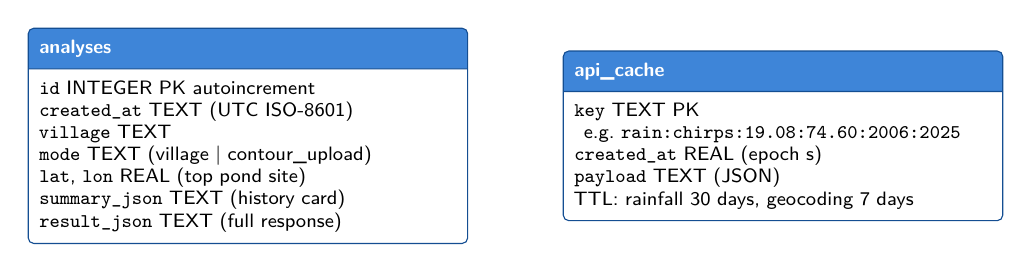
\begin{tikzpicture}[font=\sffamily\scriptsize,
  tbl/.style={rectangle split,rectangle split parts=2,draw=accent!70!black,rounded corners=2pt,
    rectangle split part fill={accent!85,white},align=left,inner sep=4pt,text width=5.3cm}]
\node[tbl] (a) {\textcolor{white}{\textbf{analyses}}
\nodepart{two}\texttt{id} INTEGER PK autoincrement\\ \texttt{created\_at} TEXT (UTC ISO-8601)\\ \texttt{village} TEXT\\ \texttt{mode} TEXT (village | contour\_upload)\\ \texttt{lat}, \texttt{lon} REAL (top pond site)\\ \texttt{summary\_json} TEXT (history card)\\ \texttt{result\_json} TEXT (full response)};
\node[tbl,right=1.2cm of a] (c) {\textcolor{white}{\textbf{api\_cache}}
\nodepart{two}\texttt{key} TEXT PK\\ \phantom{x}e.g.\ \texttt{rain:chirps:19.08:74.60:2006:2025}\\ \texttt{created\_at} REAL (epoch s)\\ \texttt{payload} TEXT (JSON)\\ TTL: rainfall 30 days, geocoding 7 days};
\end{tikzpicture}
\caption{SQLite schema. An index on \texttt{analyses(created\_at)} serves the history list.}
\label{fig:schema}
\end{figure}

\subsection{Key design decisions}
Table~\ref{tab:decisions} records the main design choices, the alternatives considered and the
reasons. They are the decisions most likely to be questioned, so each is justified by a
requirement or by measured evidence.

\begin{table}[H]
\centering\small
\caption{Design decisions and rationale.}
\label{tab:decisions}
\begin{tabularx}{\textwidth}{@{}>{\raggedright\arraybackslash}p{2.7cm}>{\raggedright\arraybackslash}p{3.0cm}Y@{}}
\toprule
Decision & Alternatives & Rationale \\
\midrule
FastAPI & Flask, Django & Pydantic models give request validation and an OpenAPI/Swagger reference for free (deliverable: API documentation); async-capable; the same schemas document and validate. \\
NumPy / SciPy / OpenCV hydrology, no GDAL & GDAL, WhiteboxTools, GRASS & Installs from pip wheels on any platform and on free hosting; every algorithm is visible and testable. The algorithms are standard and small enough to implement directly. \\
Terrain tiles for the DEM & OpenTopography, Open-Elevation, SRTM downloads & One HTTP request per 256$\times$256 tile, global, key-less and cacheable. A point-sampling API would need \num{40000} queries for a \num{200}$\times$\num{200} grid. \\
Local equirectangular projection & UTM via \texttt{pyproj} & Distortion is far below the DEM error over a few kilometres; avoids a PROJ dependency. \\
CHIRPS as default rainfall & Open-Meteo ERA5, NASA POWER, IMD grids & Best agreement with IMD normals (Section~\ref{sec:val-rain}); IMD grids are bulk files, not an API. The others are kept as fallbacks. \\
Daily SCS-CN & Rational method, monthly water balance & Captures storm-size non-linearity and antecedent moisture; the standard in Indian watershed manuals. Rational method kept as a cross-check. \\
OpenCV rules + OSM for land & Deep segmentation model & No labelled training data for Indian villages; rule-based indices are explainable, need no GPU, and reached 92\,\% accuracy (Section~\ref{sec:val-land}). \\
SQLite & PostgreSQL, MongoDB & The data is a small document store with no concurrent writers; zero administration. The \texttt{db.py} interface isolates the choice. \\
Leaflet + vanilla JS & React, Mapbox GL & The brief asks for a basic front-end library; no build step; small bundle. \\
\bottomrule
\end{tabularx}
\end{table}

% =====================================================================
\section{Methodology}\label{sec:method}
% =====================================================================
\subsection{Terrain model}
\paragraph{Grid and projection.} For a village centre $(\lambda_0,\varphi_0)$ and radius $R$
(default \SI{2}{km}) a square grid of $N\times N$ cells (default $N=200$, cell size
$\Delta=2R/N=\SI{20}{m}$) is defined in a local equirectangular projection:
\begin{equation}
x = R_E\cos\varphi_0\,(\lambda-\lambda_0)\frac{\pi}{180},\qquad
y = R_E\,(\varphi-\varphi_0)\frac{\pi}{180},
\end{equation}
with $R_E=\SI{6371008.8}{m}$. Row 0 is the southern edge.

\paragraph{Elevation.} AWS Terrain Tiles~\cite{terraintiles} encode elevation in the RGB bytes
of Web-Mercator PNG tiles:
\begin{equation}
z = 256R + G + B/256 - 32768 \quad\text{[m]}.
\end{equation}
The tiles covering the grid are downloaded in parallel, decoded with OpenCV and stitched. The
elevation mosaic is then sampled at every cell centre with \code{cv2.remap} using bilinear
interpolation. Decoding happens \emph{before} resampling: interpolating the packed bytes would
mix the high and low bytes of neighbouring pixels and produce errors of hundreds of metres.

\paragraph{Contour-map input.} For uploaded KML/KMZ maps, the elevation of each contour is
detected by trying four strategies in order: coordinate $z$ values, \code{ExtendedData}, the
placemark name, then the folder name. A strategy is accepted only if it covers at least 90\,\%
of lines and yields varying values. The contour vertices are then linearly interpolated over
their Delaunay triangulation, with nearest-neighbour fill outside the convex hull.

\subsection{Flow routing}
\paragraph{Depression filling.} Interpolated DEMs contain spurious pits that trap routed water.
The Priority-Flood algorithm~\cite{barnes2014} seeds a priority queue with all edge cells and
repeatedly pops the lowest cell, raising each unvisited neighbour to at least the popped
elevation plus $\varepsilon=10^{-4}$\,m. This yields a surface in which every cell has a
monotone downhill path to the edge, in $O(n\log n)$.

\paragraph{D8 directions.} Each cell drains to the neighbour $k$ maximising the distance-weighted
drop~\cite{ocallaghan1984}
\begin{equation}
s_k = \frac{z_c - z_k}{d_k},\qquad d_k\in\{1,\sqrt2\}\,\Delta,
\end{equation}
and is marked as draining off-grid if no $s_k>0$. The computation is vectorised as eight
shifted array comparisons.

\paragraph{Flow accumulation.} Cells are visited in decreasing filled elevation; each adds its
count to its downstream neighbour. Because flow is strictly downhill on the filled surface, a
cell's total is final before it is passed on. This removes any need for recursion or graph
sorting.

\paragraph{Catchment delineation and boundary.} The catchment of an outlet is found by
breadth-first traversal of the \emph{reversed} D8 graph. Its boundary is traced by collecting
every cell edge that separates catchment from non-catchment, stitching the edges into a ring,
and dropping collinear vertices. The polygon therefore follows exact cell edges, and its
shoelace area equals the cell count times $\Delta^2$, which a unit test verifies.

\paragraph{Edge-inflow detection.} A catchment that extends beyond the map would be
underestimated. A border cell whose D8 direction points \emph{into} the grid sits on ground
sloping inward from the edge, so land beyond the edge probably drains in. All cells downstream
of such a cell are flagged by a highest-first propagation analogous to accumulation. In village
mode flagged cells are excluded from siting, which guarantees complete catchments.

\subsection{Land availability}\label{sec:land}
Three independent evidence layers are rasterised onto the analysis grid.

\paragraph{Satellite classification (OpenCV).} Esri World Imagery is resampled to a grid four
times finer than the DEM (\SI{5}{m}). Each pixel is classified as follows.
\begin{itemize}
  \item \emph{Vegetation}: pixels where the Green--Red Vegetation Index
        $\mathrm{GRVI}=(G-R)/(G+R)$~\cite{tucker1979,motohka2010} exceeds a threshold
        $\tau$. The threshold is chosen per image by Otsu's method~\cite{otsu1979} and clamped
        to $[0,0.10]$ so that an almost uniformly bare or green scene is not split in half.
  \item \emph{Built-up}: clusters of bright, highly textured pixels. A pixel is a candidate if
        its local standard deviation over \SI{15}{m} exceeds
        $\max(18,\;P_{90})$ and its brightness exceeds the median. It is built-up if the
        candidate density over a \SI{40}{m} window exceeds 0.30. The density test separates
        villages from isolated field boundaries.
  \item \emph{Water}: dark ($V<90$), blue-dominant and smooth pixels.
  \item \emph{Open land}: everything else.
\end{itemize}
Morphological opening and closing (\SI{5}{px} ellipse) remove speckle. Class fractions per DEM
cell are obtained by area-averaging with \code{INTER\_AREA}.

\paragraph{OpenStreetMap.} One Overpass query retrieves buildings, roads, railways, waterways,
land use, natural features, amenities and protected areas. Features are burned into masks with
\code{cv2.fillPoly} and \code{cv2.polylines}, with safety buffers: \SI{20}{m} around buildings
and \SIrange{4}{30}{m} around roads depending on class. Multipolygon relations are stitched
from their member ways. Settlements, institutions, forest, water bodies and rivers are
excluded. Grassland, scrub, meadow, village green or public-ownership tags mark land as
\emph{preferred}, since in Indian villages such land is usually common or government land.
Farmland remains allowed but is ranked lower.

\paragraph{Parcels and slope.} If the administrator draws or uploads government land parcels,
siting is restricted to them. Finally, ground steeper than a threshold (default \ang{8}) is
excluded. The result is a boolean \emph{allowed} mask, a land tier (preferred / open /
farmland / excluded) and a land score in $[0,1]$.

\subsection{Site scoring and ranking}
Within the interior of the grid (excluding a 6\,\% border and edge-inflow cells), the
candidates are allowed cells on the drainage network. The drainage threshold is the 92nd
percentile of accumulation, relaxed in steps to the 60th if available land does not reach the
main channels. Each candidate $c$ receives the score
\begin{equation}
S_c = 0.75\big(0.45\,\hat{A}_c + 0.35\,(1-\hat{\theta}_c) + 0.20\,\hat{\kappa}_c\big) + 0.25\,L_c,
\label{eq:score}
\end{equation}
where $\hat{A}$ is the min--max normalised $\log(1+\text{accumulation})$, $\hat\theta$ the
normalised slope, $\hat\kappa$ the normalised concavity (negative Laplacian) and $L$ the land
score. The weights encode the priorities of pond siting: water must arrive, excavation must be
stable, and hollows hold water naturally.

Taking the top five scores would return five adjacent cells on one stream.
Algorithm~\ref{alg:rank} instead enforces spatial separation and hydrological independence:
no candidate may lie upstream or downstream of another, so each pond harvests a different part
of the landscape and their inflows can be summed without double counting.

\begin{algorithm}[H]
\caption{Ranking independent candidate sites}\label{alg:rank}
\begin{algorithmic}[1]
\Require score grid $S$, D8 directions $D$, number $n$, minimum separation $d_{\min}$
\State $\mathcal{A}\gets[\,]$; $\mathcal{M}\gets[\,]$ \Comment{accepted sites, their catchment masks}
\ForAll{cells $c$ in decreasing order of $S$}
  \State \textbf{if} $|\mathcal{A}|=n$ \textbf{then break}
  \State \textbf{if} $\exists a\in\mathcal{A}:\ \lVert c-a\rVert<d_{\min}$ \textbf{then continue} \Comment{too close}
  \State \textbf{if} $\exists m\in\mathcal{M}:\ m[c]$ \textbf{then continue} \Comment{$c$ upstream of an accepted site}
  \State $m_c\gets\textsc{Catchment}(D,c)$
  \State \textbf{if} $\exists a\in\mathcal{A}:\ m_c[a]$ \textbf{then continue} \Comment{$c$ downstream of an accepted site}
  \State append $c$ to $\mathcal{A}$ and $m_c$ to $\mathcal{M}$
\EndFor
\State \Return $\mathcal{A}$
\end{algorithmic}
\end{algorithm}

A user-chosen location is snapped to the highest-accumulation cell within a \SI{60}{m} radius
(on allowed land if possible). It becomes rank 1, and the automatic sites follow as
alternatives.

\subsection{Rainfall}
\paragraph{Sources.} Precipitation is taken, in order of preference, from:
\begin{enumerate}
  \item CHIRPS v2.0~\cite{funk2015}, a \ang{0.05} daily product that blends satellite estimates
        with rain-gauge data, accessed through NASA/USAID SERVIR ClimateSERV in parallel
        ten-year chunks;
  \item Open-Meteo's ERA5 reanalysis~\cite{hersbach2020};
  \item NASA POWER~\cite{gelaro2017}.
\end{enumerate}
Reference evapotranspiration ET$_0$ comes from Open-Meteo (FAO-56 Penman--Monteith) or is
computed from NASA POWER temperatures by Hargreaves--Samani~\cite{hargreaves1985}:
\begin{equation}
\mathrm{ET}_0 = 0.0023\,(0.408R_a)\,(T_{\text{mean}}+17.8)\sqrt{T_{\max}-T_{\min}},
\end{equation}
with extraterrestrial radiation $R_a$ from FAO-56 eq.~21~\cite{allen1998}. If the
administrator enters a known long-term normal $\bar P^\ast$, the daily series is linearly
scaled by $\bar P^\ast/\bar P$. This preserves the storm pattern while removing the bias.

\paragraph{Statistics.} The following statistics are computed from the daily series: mean,
median, standard deviation and coefficient of variation of annual totals; the 75\,\%-dependable
rainfall (25th percentile of annual totals, i.e.\ equalled or exceeded three years in four);
the driest and wettest years; rainy days ($\geq\SI{2.5}{mm}$, the IMD definition); the heaviest
day; the monsoon share (June--September); monthly climatology; and annual and dry-season
(October--May) ET$_0$.

\subsection{Runoff}\label{sec:runoff}
Runoff is simulated for every day of the record with the SCS Curve Number
method~\cite{tr55}:
\begin{equation}
S=\frac{25400}{CN}-254,\qquad I_a=0.2S,\qquad
Q=\begin{cases}\dfrac{(P-I_a)^2}{P-I_a+S}, & P>I_a\\[4pt] 0, & \text{otherwise}\end{cases}
\qquad[\text{mm}].
\end{equation}
Curve numbers (Table~\ref{tab:cn}) are assigned per land-cover class for the chosen hydrologic
soil group. Runoff is computed per class and area-weighted over the catchment's land-cover
fractions. This is more accurate than applying a single composite CN, because the equation is
non-linear. Each day's CN is adjusted for antecedent moisture from the preceding five days'
rainfall $P_5$: AMC\,I if $P_5<\SI{35.6}{mm}$, AMC\,III if $P_5>\SI{53.3}{mm}$, using Hawkins'
conversions~\cite{hawkins1985}
\begin{equation}
CN_{\mathrm{I}}=\frac{CN}{2.281-0.01281\,CN},\qquad CN_{\mathrm{III}}=\frac{CN}{0.427+0.00573\,CN}.
\end{equation}
Annual volumes are $V=Q\cdot A$. The mean and the 75\,\%-dependable (25th percentile) annual
volumes are reported. The rational method $V=A\bar P C$, with a land-cover-weighted $C$, is
reported alongside as a cross-check.

\begin{table}[H]
\centering\small
\caption{Curve numbers (AMC II) by land-cover class and hydrologic soil group, after TR-55.}
\label{tab:cn}
\begin{tabular}{@{}llcccc c@{}}
\toprule
Class & TR-55 cover type & A & B & C & D & Rational $C$\\
\midrule
Water & rain on water surface & 98 & 98 & 98 & 98 & 1.00\\
Built-up & residential, $\approx$85\,\% impervious & 89 & 92 & 94 & 95 & 0.75\\
Vegetation & row crops, straight row, good & 67 & 78 & 85 & 89 & 0.25\\
Open land & pasture/fallow, poor & 68 & 79 & 86 & 89 & 0.35\\
Forest (OSM) & woods, fair & 36 & 60 & 73 & 79 & 0.15\\
\bottomrule
\end{tabular}
\end{table}

\subsection{Pond design}\label{sec:pond}
The pond is a rectangular excavated frustum with side slope $z$\,H\,:\,1\,V (default 1.5),
length $1.5\times$ width, with the long side laid along the contour, i.e.\ perpendicular to
the local gradient. For top width $W$, length $L$ and depth $d$, the volume is given exactly
by the prismoidal formula
\begin{equation}
V=\frac{d}{6}\Big(LW + 4(L-zd)(W-zd) + (L-2zd)(W-2zd)\Big),
\end{equation}
and $W$ is found for a target $V$ by bisection. The design procedure is:
\begin{enumerate}
  \item \textbf{Target storage} $V^\ast = f\cdot V_{75}$, with $f=0.5$ by default. The pond
        then fills about twice in a dependable (dry) year, leaving margin for evaporation,
        seepage and a weak early monsoon.
  \item \textbf{Depth.} Start at \SI{3}{m}, the depth used in MGNREGA and Amrit Sarovar
        designs~\cite{amritsarovar}. If the footprint (including \SI{0.5}{m} freeboard)
        exceeds 80\,\% of the connected patch of available land at the site, or the
        \SI{2}{ha} village-pond cap, increase the depth in \SI{0.5}{m} steps up to
        \SI{4.5}{m}. Deeper ponds also lose proportionally less water to evaporation.
  \item \textbf{Capping.} If the pond still does not fit, reduce the volume to what fits and
        say so.
  \item \textbf{Small ponds.} Reduce the depth (down to \SI{2}{m}) so that the bed stays at
        least \SI{4}{m} wide for machinery.
\end{enumerate}
The procedure also reports:
\begin{itemize}
  \item excavation volume;
  \item dry-season open-water evaporation $E=1.05\,\mathrm{ET}_{0,\text{Oct--May}}\cdot A_{\text{mid}}$,
        where $A_{\text{mid}}$ is the water surface at half depth~\cite{allen1998};
  \item four-month seepage at a rate that depends on soil group (1--10\,mm/day),
        with lining advice for soil groups A and B;
  \item fills per dependable year.
\end{itemize}

\begin{figure}[H]
\centering
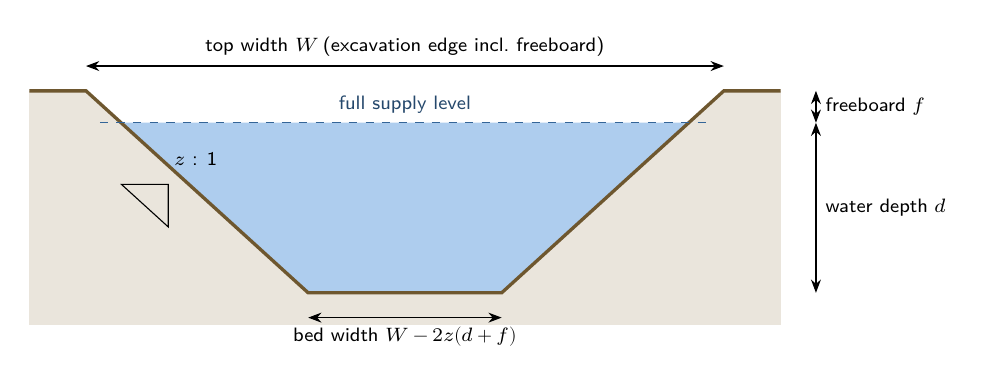
\begin{tikzpicture}[scale=0.9,font=\sffamily\scriptsize]
\def\W{9} \def\d{2.4} \def\z{1.1} \def\f{0.45}
\fill[soil!18] (-0.8,0) -- (\W+0.8,0) -- (\W+0.8,-\d-0.9) -- (-0.8,-\d-0.9) -- cycle;
\fill[white] (0,0) -- (\z*\d+\z*\f,-\d-\f) -- (\W-\z*\d-\z*\f,-\d-\f) -- (\W,0) -- cycle;
\fill[water!45] (\z*\f,-\f) -- (\z*\d+\z*\f,-\d-\f) -- (\W-\z*\d-\z*\f,-\d-\f) -- (\W-\z*\f,-\f) -- cycle;
\draw[soil!80!black,line width=1.2pt] (-0.8,0) -- (0,0) -- (\z*\d+\z*\f,-\d-\f) -- (\W-\z*\d-\z*\f,-\d-\f) -- (\W,0) -- (\W+0.8,0);
\draw[water!70!black,dashed] (\z*\f-0.3,-\f) -- (\W-\z*\f+0.3,-\f);
\node[water!50!black,anchor=south] at (\W/2,-\f) {full supply level};
\draw[{Stealth}-{Stealth}] (0,0.35) -- node[above]{top width $W$ (excavation edge incl.\ freeboard)} (\W,0.35);
\draw[{Stealth}-{Stealth}] (\z*\d+\z*\f,-\d-\f-0.35) -- node[below]{bed width $W-2z(d+f)$} (\W-\z*\d-\z*\f,-\d-\f-0.35);
\draw[{Stealth}-{Stealth}] (\W+1.3,-\f) -- node[right]{water depth $d$} (\W+1.3,-\d-\f);
\draw[{Stealth}-{Stealth}] (\W+1.3,0) -- node[right]{freeboard $f$} (\W+1.3,-\f);
\draw (0.5,-0.55*\d) -- ++(\z*0.6,-0.6) -- ++(0,0.6) -- cycle;
\node at (1.55,-0.4*\d) {$z$ : 1};
\end{tikzpicture}
\caption{Cross-section of the excavated pond, showing the design variables.}
\label{fig:section}
\end{figure}

% =====================================================================
\section{Implementation}
% =====================================================================
\subsection{Code organisation}
The back end comprises about \num{3400} lines of Python in fourteen modules
(Table~\ref{tab:modules}). The front end is about \num{1200} lines of HTML, CSS and JavaScript,
and there are about \num{220} lines of tests. Modules are layered: \code{main.py} handles only
HTTP concerns; \code{pipeline.py} orchestrates; each analysis module is a pure function of
arrays and parameters and is independently testable; I/O is confined to \code{tiles.py},
\code{rainfall.py}, \code{landcover.fetch\_osm}, \code{geocode.py} and \code{db.py}.

\begin{table}[H]
\centering\small
\caption{Back-end modules.}
\label{tab:modules}
\begin{tabularx}{\textwidth}{@{}lrY@{}}
\toprule
Module & Lines & Responsibility \\
\midrule
\code{main.py} & 236 & FastAPI routes, request validation, error mapping, static front end \\
\code{schemas.py} & 98 & Pydantic request/response models; drive the OpenAPI documentation \\
\code{pipeline.py} & 334 & Orchestration; per-candidate evaluation; result assembly; persistence \\
\code{tiles.py} & 164 & Web-Mercator maths, parallel tile download, disk cache, OpenCV mosaic and \code{remap} \\
\code{elevation.py} & 91 & DEM from terrain tiles, with Open-Meteo elevation fallback \\
\code{terrain.py} & 197 & Projection, DEM grid, contour interpolation, slope and curvature \\
\code{kml\_parser.py} & 225 & KML/KMZ parsing with four elevation-detection strategies \\
\code{hydrology.py} & 239 & Priority-Flood, D8, accumulation, edge inflow, catchment, boundary \\
\code{landcover.py} & 457 & OpenCV classification, Overpass query, rasterisation, parcels, tiers \\
\code{pond.py} & 259 & Site scoring, candidate ranking, snapping, natural-basin storage \\
\code{rainfall.py} & 340 & CHIRPS/Open-Meteo/NASA clients, parallel fetch, cache, scaling, statistics \\
\code{runoff.py} & 150 & Curve numbers, AMC adjustment, daily SCS-CN, rational method \\
\code{design.py} & 184 & Frustum geometry, depth selection, losses, footprint polygon \\
\code{layers.py} & 262 & Contours, drainage network, land polygons, PNG overlays \\
\code{db.py} & 112 & SQLite persistence and API cache \\
\bottomrule
\end{tabularx}
\end{table}

\subsection{Performance}
Table~\ref{tab:timing} shows the stage timings for Hiware Bazar on a laptop. Terrain analysis
on \num{40000} cells takes about \SI{60}{ms} because D8 is vectorised and accumulation is a
single sorted pass. The first run for a location is dominated by the CHIRPS download (about
\SI{35}{s} for two parallel ten-year requests). Repeat runs use the cache and take about
\SI{2.5}{s}.

\begin{table}[H]
\centering\small
\caption{Stage timings, Hiware Bazar (cached run; first run adds $\approx$\SI{35}{s} of rainfall download).}
\label{tab:timing}
\begin{tabular}{@{}lr@{}}
\toprule
Stage & Time (s)\\
\midrule
Fill, D8, accumulation, edge inflow & 0.062\\
Land assessment (imagery classification + OSM) & 1.524\\
Scoring and ranking 5 candidates & 0.066\\
Rainfall (cache) & 0.752\\
Catchments, runoff and design for 5 candidates & 0.047\\
Map layers & 0.022\\
\midrule
\textbf{Total server time} & \textbf{2.47}\\
\bottomrule
\end{tabular}
\end{table}

\subsection{Robustness}
Every external dependency has a defined failure mode.
\begin{itemize}
  \item Terrain tiles fall back to the Open-Meteo elevation API.
  \item Rainfall falls back through three providers. Transient network errors are retried with
        back-off; definitive errors such as rate limits move straight to the next source.
  \item If imagery or OpenStreetMap is unavailable, siting continues on the remaining evidence.
  \item If all rainfall services fail, the rational method is applied to a fallback rainfall
        value.
\end{itemize}
In every case the degradation appears in the response's \code{warnings} array and on screen.
Validation errors return HTTP 422, upstream outages 502, and all errors share the JSON shape
\code{\{"status":"error","detail":...\}}.

\subsection{Front end}
The front end is a single page with Village, Contour file and History tabs. The Village tab
provides:
\begin{itemize}
  \item village search;
  \item a preview of the analysis area;
  \item parcel drawing and upload (Leaflet.draw);
  \item an optional manual pond pin;
  \item advanced parameters: soil group, rainfall dataset and normal, storage fraction and
        depth limits.
\end{itemize}
While an analysis runs, a staged progress overlay covers the map. The results comprise:
\begin{itemize}
  \item a headline storage card and four key indicators;
  \item the ranked candidate table, also shown as numbered map markers, where selecting a
        candidate re-renders everything for it;
  \item Pond, Rainfall, Runoff and Site~\&~land sub-tabs with a pond cross-section and charts;
  \item map overlays for contours, drainage, catchment, available land, land-cover and relief
        rasters, and pond footprints;
  \item JSON and GeoJSON export and a print stylesheet for a paper report.
\end{itemize}
Accessibility work included ARIA tab semantics, keyboard-operable lists and table rows, visible
focus outlines, a skip link, labelled map and chart regions, a reduced-motion mode, and a text
colour raised to a 5.6:1 contrast ratio (WCAG AA).

\begin{figure}[H]
\centering
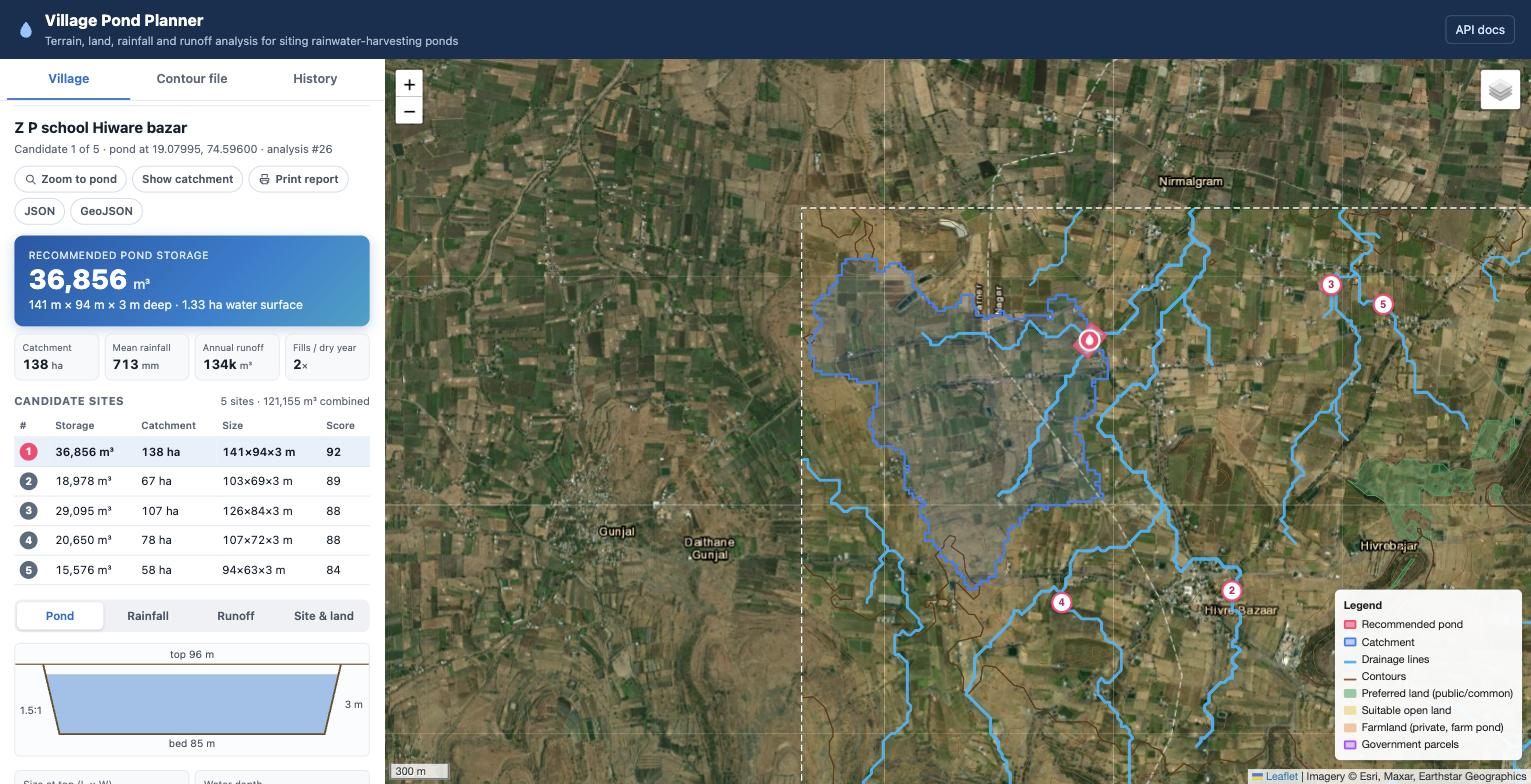
\includegraphics[width=\textwidth]{../docs/app_screenshot.jpg}
\caption{Results for Hiware Bazar: candidate~1 with its catchment (blue), drainage network,
contours and candidates 2--5 (numbered markers). The sidebar shows the headline storage,
indicators and the ranked candidate table.}
\label{fig:ui}
\end{figure}

% =====================================================================
\section{Results: Hiware Bazar case study}
% =====================================================================
Hiware Bazar (Ahilyanagar district, Maharashtra) is a well-known model village for watershed
development on the semi-arid Deccan plateau, in the rain shadow of the Western Ghats. The
analysis covered a \SI{4}{km}$\times$\SI{4}{km} area centred at \ang{19.0680}\,N,
\ang{74.6012}\,E, with soil group C and default parameters.

\subsection{Terrain and land}
The DEM spans \SIrange{692}{875}{m}. OpenStreetMap supplied 111 buildings, 39 roads and 23 water
features. After exclusions and the \ang{8} slope limit, 76\,\% of the area
(\SI{1219}{ha}) is suitable, of which \SI{24.4}{ha} carries tags that suggest common land.
Figure~\ref{fig:landcover} shows the classification: the village core is correctly identified
as built-up, and irrigated plots as vegetation within largely open, fallow terrain.

\begin{figure}[H]
\centering
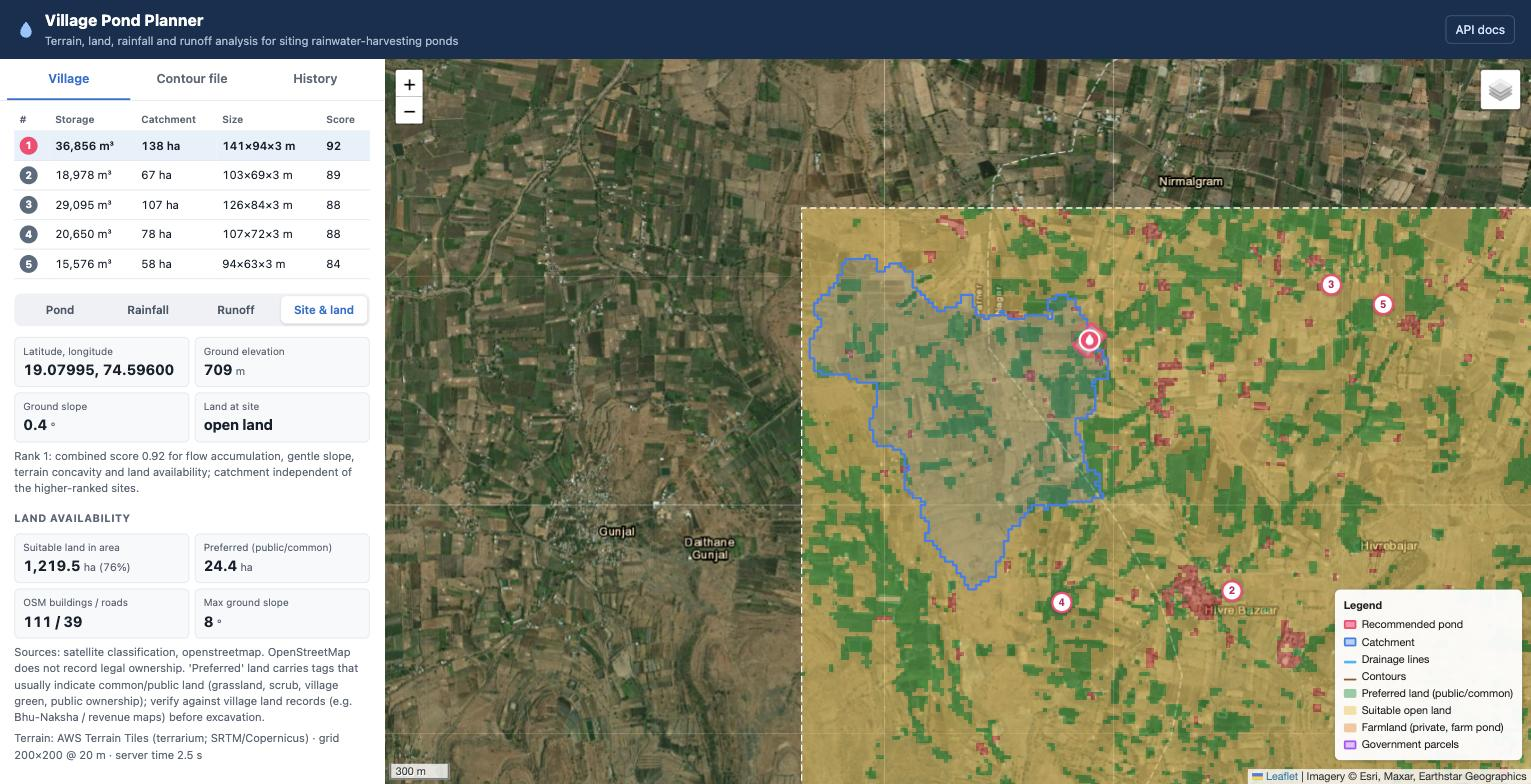
\includegraphics[width=\textwidth]{../docs/landcover_overlay.jpg}
\caption{Land-cover classification overlay (green: vegetation, yellow: open land, red:
built-up) with candidate~1's catchment. The Hiware Bazaar settlement (lower right) is detected
as built-up and excluded.}
\label{fig:landcover}
\end{figure}

\subsection{Rainfall}
CHIRPS gives a mean of \SI{713}{mm} for 2006--2025 (Figure~\ref{fig:caserain}). The
75\,\%-dependable rainfall is \SI{599}{mm}, and the coefficient of variation of 23\,\% shows
typical Deccan variability: from \SI{373}{mm} in 2018 to \SI{1063}{mm} in 2020. The site
records 53 rainy days a year, and 79\,\% of the rain falls between June and September. The
heaviest day recorded is \SI{78}{mm}. Reference evapotranspiration is \SI{1771}{mm/yr}, of
which \SI{1249}{mm} falls in the October--May dry season.

\begin{figure}[H]
\centering
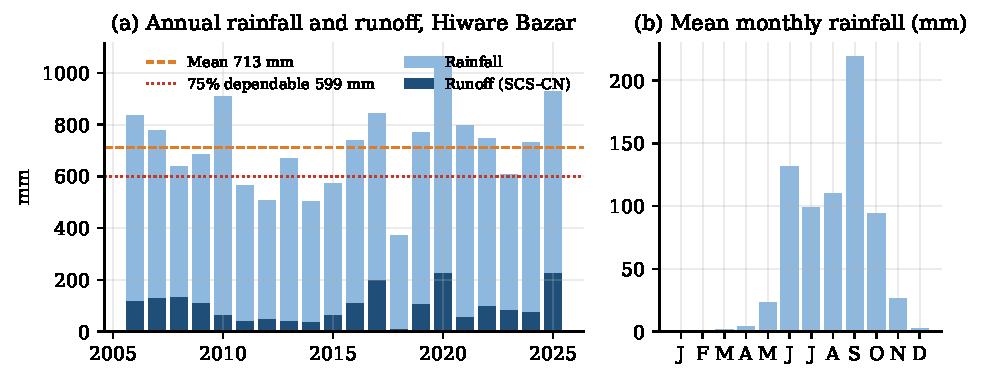
\includegraphics[width=\textwidth]{figures/case_rainfall.pdf}
\caption{Hiware Bazar: (a) annual rainfall and simulated runoff depth, 2006--2025; (b) monthly
climatology.}
\label{fig:caserain}
\end{figure}

\subsection{Candidate sites}
Algorithm~\ref{alg:rank} found five hydrologically independent sites (Figure~\ref{fig:cands},
Table~\ref{tab:cands}), all on open land with slopes of \ang{0.1}--\ang{1.6}. Their combined
storage is \SI{121155}{\cubic\metre}.

\begin{figure}[H]
\centering
\begin{subfigure}[b]{0.56\textwidth}\centering
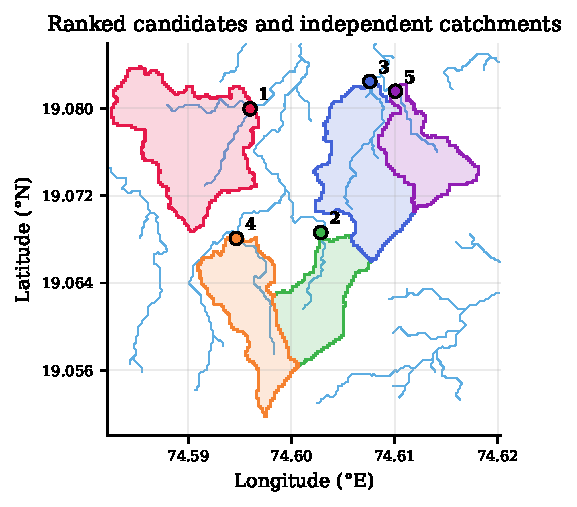
\includegraphics[width=\textwidth]{figures/candidates.pdf}
\caption{Five ranked sites and their catchments.}
\end{subfigure}\hfill
\begin{subfigure}[b]{0.36\textwidth}\centering
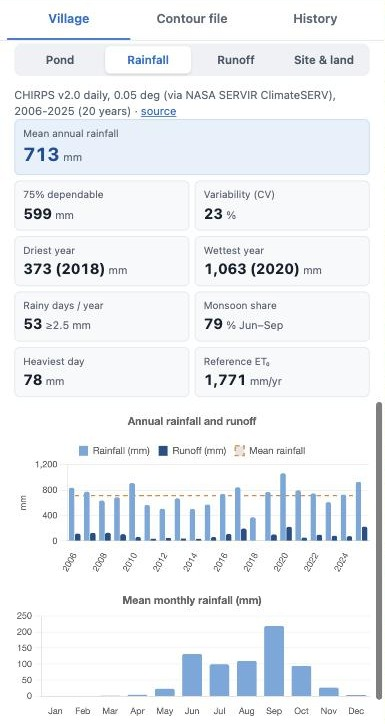
\includegraphics[width=\textwidth]{../docs/rainfall_sidebar.jpg}
\caption{Rainfall tab of the user interface.}
\end{subfigure}
\caption{Candidate sites and the rainfall interface.}
\label{fig:cands}
\end{figure}

\begin{table}[H]
\centering\small
\caption{Ranked candidate ponds for Hiware Bazar (soil group C, CHIRPS 2006--2025).}
\label{tab:cands}
\begin{tabular}{@{}c c c r r r r c r@{}}
\toprule
Rank & Score & Location (°N, °E) & Catch. & Mean runoff & Dep.\ runoff & Storage & Top size & Earthwork \\
 & & & (ha) & (\mcube/yr) & (\mcube/yr) & (\mcube) & (m) & (\mcube) \\
\midrule
1 & 0.92 & 19.07995, 74.59600 & 137.6 & \num{134368} & \num{73712} & \num{36856} & 141$\times$94 & \num{43604}\\
2 & 0.89 & 19.06862, 74.60285 & 67.3 & \num{68007} & \num{37955} & \num{18978} & 103$\times$69 & \num{22578}\\
3 & 0.88 & 19.08247, 74.60760 & 106.5 & \num{105393} & \num{58190} & \num{29095} & 126$\times$84 & \num{34483}\\
4 & 0.88 & 19.06808, 74.59466 & 78.5 & \num{75657} & \num{41301} & \num{20650} & 107$\times$72 & \num{24548}\\
5 & 0.84 & 19.08157, 74.61008 & 57.7 & \num{56694} & \num{31153} & \num{15576} & 94$\times$63 & \num{18570}\\
\midrule
\multicolumn{3}{@{}l}{\textbf{Total}} & \textbf{447.6} & \textbf{\num{440119}} & & \textbf{\num{121155}} & & \textbf{\num{143782}}\\
\bottomrule
\end{tabular}
\end{table}

\subsection{Recommended pond (rank 1)}
The top site lies at \ang{19.07995}\,N, \ang{74.59600}\,E. The ground is at \SI{709}{m} with a
slope of \ang{0.4}, on open land at the outlet of a \SI{137.6}{ha} catchment (perimeter
\SI{7.72}{km}, relief \SI{44.8}{m}, mean slope \ang{3.3}). The catchment is 77\,\% open or
fallow land, 22\,\% crops and 1\,\% built-up, giving a composite CN of 85.8. Mean runoff is
\SI{98}{mm/yr}, an effective coefficient of 0.14, or \num{134368}\,m$^3$/yr. In a
dependable year it is \SI{73712}{\cubic\metre}. Table~\ref{tab:design} summarises the design.

\begin{table}[H]
\centering\small
\caption{Recommended pond, rank 1.}
\label{tab:design}
\begin{tabular}{@{}ll@{\hspace{2.5em}}ll@{}}
\toprule
Storage capacity & \textbf{\SI{36856}{\cubic\metre}} & Water spread area & \SI{1.33}{ha}\\
Top size (L$\times$W) & \SI{141.3}{m}$\times$\SI{94.2}{m} & Excavation volume & \SI{43604}{\cubic\metre}\\
Bed size (L$\times$W) & \SI{132.3}{m}$\times$\SI{85.2}{m} & Dry-season evaporation & \SI{16099}{\cubic\metre} (44\,\%)\\
Water depth + freeboard & \SI{3.0}{m} + \SI{0.5}{m} & Seepage (4 months) & \SI{3384}{\cubic\metre}\\
Side slope & 1.5\,:\,1 & Fills per dependable year & 2.0\\
\bottomrule
\end{tabular}
\end{table}

\begin{keybox}[Interpretation]
Losing 44\,\% of storage to evaporation over the dry season is realistic for the Deccan, where
October--May ET$_0$ exceeds \SI{1.2}{m}. This is why the design favours depth over surface
area once land becomes limiting. The five candidates together could capture about 28\,\% of
the mean runoff generated by their catchments. This leaves most of the flow to continue
downstream, which avoids starving downstream users.
\end{keybox}

% =====================================================================
\section{Verification and validation}\label{sec:validation}
% =====================================================================
Verification (\emph{is the model implemented correctly?}) was done with unit tests.
Validation (\emph{does the model match reality?}) was done by comparing each data source and
classifier with an independent reference. All scripts, raw results and labelled imagery are in
the \code{validation/} directory and can be re-run.

\subsection{Unit tests}
Twenty-three \code{pytest} tests pass in 0.2\,s (Table~\ref{tab:tests}). The most informative
is the synthetic V-valley: two planes meet along a channel sloping to the south. Off-channel
cells step diagonally, so a cell at row $r$ and distance $k$ from the channel joins it at row
$r-k$. The analytic catchment of the outlet at row $r_0$ is therefore
$\{(r,c): r-|c-c_0|\ge r_0\}$. The implementation reproduces this cell for cell.

\begin{table}[H]
\centering\small
\caption{Unit tests and their independent references.}
\label{tab:tests}
\begin{tabularx}{\textwidth}{@{}lY@{}}
\toprule
Test & Reference \\
\midrule
SCS runoff, $P=\SI{100}{mm}$, CN\,80 & Hand calculation: $S=63.5$, $I_a=12.7$, $Q=87.3^2/150.8=\SI{50.54}{mm}$ \\
SCS, four further $(P,\mathrm{CN})$ pairs; zero below $I_a$ & Closed-form TR-55 equation \\
AMC conversion & Hawkins (1985): CN 75 $\rightarrow$ 56.8 (I), 87.0 (III) \\
Dry vs wet antecedent conditions & $Q_{\mathrm{I}} < Q_{\mathrm{II}} < Q_{\mathrm{III}}$ \\
Runoff volume; rational fallback & $Q\cdot A$; $A\,P\,C$ \\
Frustum volume (square, rectangle) & $\tfrac{h}{3}(A_1{+}A_2{+}\sqrt{A_1A_2})=\SI{650.67}{\cubic\metre}$; prismoidal formula by hand \\
Width solver & Round trip at three volumes \\
Pond rules & Hits target; deeper on small land; caps storage and reports it \\
Extraterrestrial radiation & FAO-56 Example 8: \ang{20}\,S, 3 Sep $\rightarrow$ \SI{32.2}{MJ.m^{-2}.d^{-1}} \\
Rainfall statistics & Constructed series with known mean, percentile, driest year, rainy days, ET$_0$ \\
Depression filling & No interior sinks; surface never lowered \\
V-valley catchment & Analytic set, cell for cell; accumulation equals its size \\
Boundary polygon & Shoelace area $=$ cell count \\
Bowl with channel; edge inflow & All cells reach the outlet; inward valley flagged, hill-top not \\
\bottomrule
\end{tabularx}
\end{table}

\subsection{Rainfall against IMD normals}\label{sec:val-rain}
For six IMD observatories in contrasting climates, each dataset's 1991--2020 mean annual
rainfall was compared with the IMD 1991--2020 normal (Figure~\ref{fig:valrain},
Table~\ref{tab:valrain}).

\begin{figure}[H]
\centering
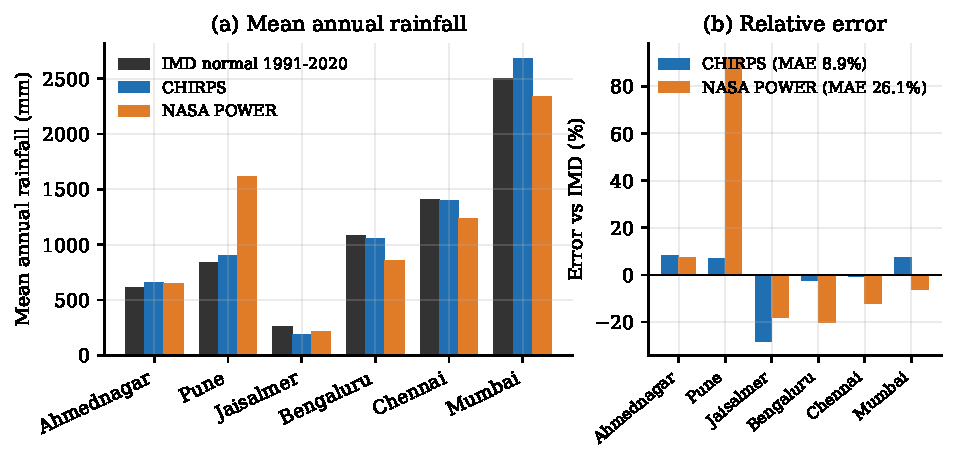
\includegraphics[width=\textwidth]{figures/rainfall_validation.pdf}
\caption{Rainfall datasets compared with IMD 1991--2020 station normals.}
\label{fig:valrain}
\end{figure}

\begin{table}[H]
\centering\small
\caption{Mean annual rainfall 1991--2020 (mm) and error relative to the IMD normal.}
\label{tab:valrain}
\begin{tabular}{@{}llrrrrr@{}}
\toprule
Station & Climate & IMD & CHIRPS & Error & NASA POWER & Error\\
\midrule
Ahmednagar & semi-arid, rain shadow & 608.1 & 658.1 & +8.2\,\% & 652.0 & +7.2\,\%\\
Pune\textsuperscript{a} & leeward Western Ghats & 841.2 & 897.9 & +6.7\,\% & 1616.7 & \textbf{+92.2\,\%}\\
Jaisalmer & arid & 256.9 & 184.8 & $-$28.1\,\% & 210.1 & $-$18.2\,\%\\
Bengaluru & semi-arid plateau & 1077.8 & 1054.0 & $-$2.2\,\% & 858.7 & $-$20.3\,\%\\
Chennai & NE-monsoon coast & 1408.4 & 1396.8 & $-$0.8\,\% & 1237.9 & $-$12.1\,\%\\
Mumbai & windward coast & 2502.3 & 2684.6 & +7.3\,\% & 2341.7 & $-$6.4\,\%\\
\midrule
\multicolumn{2}{@{}l}{Mean absolute error} & & & \textbf{8.9\,\%} & & \textbf{26.1\,\%}\\
\bottomrule
\end{tabular}\\[3pt]
{\footnotesize\textsuperscript{a}\,WMO 1991--2020 normal published by the Tokyo Climate Center from IMD observations;
other stations: IMD Climatological Tables~\cite{imdnormals}.}
\end{table}

\begin{notebox}[Finding that changed the design]
The first version of the system used Open-Meteo with a NASA POWER fallback. NASA POWER's
$\sim$\SI{50}{km} cells mix the wet windward Ghats with the dry plateau behind them, so Pune reads
almost twice its true rainfall. That dry plateau is exactly where pond planning matters. For
Hiware Bazar, NASA POWER gave \SI{910}{mm} against CHIRPS's \SI{713}{mm}, and the recommended
pond changed from \num{41298} to \SI{36856}{\cubic\metre}. CHIRPS (\ang{0.05}, calibrated
against rain gauges) was therefore made the default, and a user-supplied normal can correct any
remaining bias. CHIRPS still underestimates the desert (Jaisalmer, $-28\,\%$), a known
weakness of satellite rainfall in arid regions. Open-Meteo could not be scored because its
daily request quota for the test machine's IP had been exhausted.
\end{notebox}

\subsection{Elevation}
Terrain-tile elevations were compared with 44 OpenStreetMap summits that have an \code{ele}
tag, in three regions (Figure~\ref{fig:valdem}). The median absolute error is \SI{20}{m}, with
a systematic bias of $-\SI{27}{m}$: a \SI{30}{m} DEM averages a sharp summit with its flanks.
Summits are therefore a worst case. Pond sites lie on gentle valley floors and depend on
\emph{relative} elevation, for which the SRTM specification is \SI{10}{m} (90\,\%) and actual
errors on gentle terrain are smaller~\cite{farr2007}. The practical limitation is resolution:
features narrower than about \SI{30}{m} (bunds, drains, road embankments) are not resolved.

\begin{figure}[H]
\centering
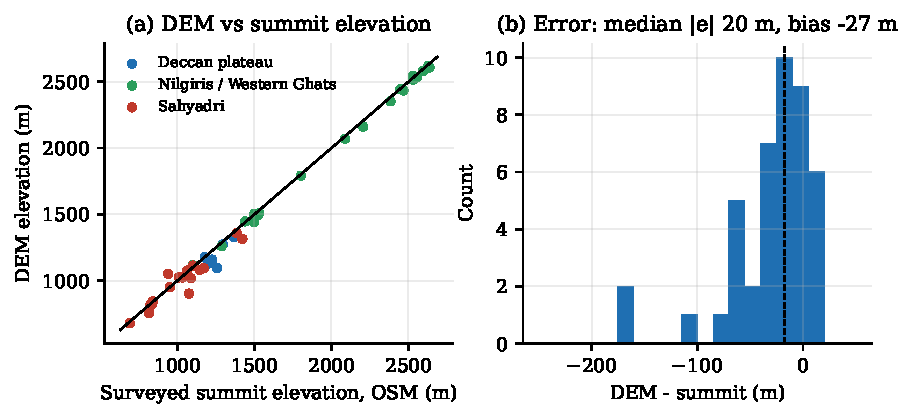
\includegraphics[width=0.92\textwidth]{figures/dem_validation.pdf}
\caption{DEM compared with surveyed summit elevations: (a) scatter; (b) error distribution.}
\label{fig:valdem}
\end{figure}

\subsection{Land-cover classifier}\label{sec:val-land}
The classifier was tested in four landscapes:
\begin{itemize}
  \item semi-arid Maharashtra;
  \item irrigated Punjab;
  \item wet Kerala (Kuttanad);
  \item arid Rajasthan.
\end{itemize}
In each, 25 of the classifier's \SI{20}{m} cells were drawn at random (seed 42). Each cell was
rendered as a \SI{100}{m} chip of zoom-18 imagery, about four times finer than the classifier
input, with the cell outlined. The classifier's output was saved separately and not shown on
the chips. Each cell was labelled by eye with its dominant cover. Cells split roughly evenly
between two covers were marked mixed and excluded (13 of 100). Accuracy was assessed following
Congalton~\cite{congalton1991}, with Cohen's $\kappa$~\cite{cohen1960} for agreement beyond
chance.

\begin{figure}[H]
\centering
\begin{minipage}[c]{0.42\textwidth}\centering
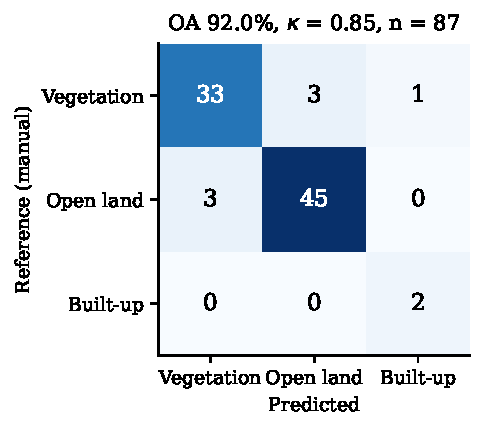
\includegraphics[width=\textwidth]{figures/landcover_confusion.pdf}
\end{minipage}\hfill
\begin{minipage}[c]{0.54\textwidth}\small
\begin{tabular}{@{}lcc@{}}
\toprule
Site & Correct & Accuracy\\
\midrule
Hiware Bazar (semi-arid) & 20/21 & 95\,\%\\
Ludhiana (irrigated) & 20/20 & 100\,\%\\
Kuttanad (wet) & 21/23 & 91\,\%\\
Jaipur rural (arid) & 19/23 & 83\,\%\\
\midrule
\textbf{All} & \textbf{80/87} & \textbf{92\,\%}\\
\bottomrule
\end{tabular}\\[6pt]
Producer's accuracy: vegetation 89\,\%, open land 94\,\%.\\
User's accuracy: vegetation 92\,\%, open land 94\,\%.
\end{minipage}
\caption{Land-cover confusion matrix and per-site accuracy (87 unmixed cells).}
\label{fig:valland}
\end{figure}

The errors fall into three groups:
\begin{itemize}
  \item Three are pale-green sparse grass in arid Rajasthan, which GRVI calls vegetation. That
        is a borderline case with little consequence for siting.
  \item Two are cells with a single tree covering about half of the cell.
  \item Random sampling drew only two built-up cells and no water cells, so the accuracy of
        those classes is not established by this sample.
\end{itemize}
In the system, buildings, roads and water bodies are primarily excluded from OpenStreetMap
with safety buffers; the satellite classes provide a secondary safeguard.

\subsection{Sensitivity analysis}
The sensitivity of runoff to its two most uncertain inputs was explored on the real Hiware
Bazar series (Figure~\ref{fig:sens}). Runoff responds to rainfall with an elasticity of about
three: $\pm10\,\%$ rainfall changes runoff by $-30\,\%$ and $+31\,\%$. A rational-method model
would predict a proportional $\pm10\,\%$. Soil group is even more influential: from group A to
group D, runoff rises from \num{37301} to \num{176527}\,m$^3$/yr, a factor of 4.7. The
two inputs that matter most are therefore the rainfall dataset, which is why it was validated
and made correctable, and the soil group. The soil group is exposed as a parameter with plain
descriptions (e.g.\ ``black cotton soil'' for D) because it cannot be inferred from imagery.

\begin{figure}[H]
\centering
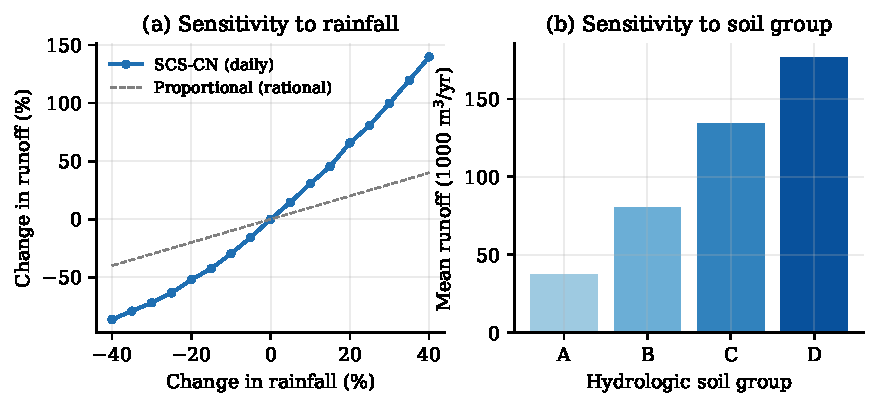
\includegraphics[width=0.92\textwidth]{figures/sensitivity.pdf}
\caption{Sensitivity of mean annual runoff at Hiware Bazar (rank 1): (a) to a uniform scaling of
daily rainfall; (b) to hydrologic soil group.}
\label{fig:sens}
\end{figure}

\subsection{What has not been validated}
\begin{itemize}
  \item Runoff volumes against measured stream flow: no gauged village-scale catchments exist
        in open data.
  \item Catchment boundaries against official micro-watershed maps (e.g.\ Bhuvan).
  \item Legal land ownership, which is absent from open data.
  \item Siting against locations chosen by engineers, which would be possible with MGNREGA or
        Amrit Sarovar site records.
\end{itemize}

% =====================================================================
\section{Software quality and project management}
% =====================================================================
\begin{description}[style=nextline,leftmargin=1.2em]
  \item[Modularity] Each analysis stage is a separate module with a narrow, array-based
        interface; the pipeline composes them. Adding a terrain source, rainfall provider or
        land-evidence layer touches one module.
  \item[Typing and validation] Type hints throughout; Pydantic models validate every request
        (ranges, enumerations) and generate the OpenAPI reference at \code{/docs}.
  \item[Testing] Unit tests cover all formulas and the hydrology core; validation scripts cover
        the data sources. Both can be re-run with one command.
  \item[Traceability] Every response carries its data sources, methods, parameters, candidate
        ranking rule and per-stage timings in \code{method}, plus any degradations in
        \code{warnings}.
  \item[Reproducibility] Pinned dependencies (\code{requirements.txt},
        \code{requirements-dev.txt}), a Dockerfile, deterministic random seeds in validation,
        and figures regenerated from saved results by \code{report/figures/make\_figures.py}.
  \item[Configuration] Environment variables only (\code{MAPTILER\_KEY},
        \code{DATABASE\_PATH}, \code{TILE\_CACHE\_DIR}); no secrets in the code; \code{.env}
        excluded from version control.
  \item[Deployment] Container-ready (Docker) and deployable on free platforms such as Render
        with a persistent disk for the database.
\end{description}

% =====================================================================
\section{Limitations and future work}
% =====================================================================
\begin{itemize}
  \item \textbf{Resolution.} The $\sim$\SI{30}{m} DEM cannot see small bunds or drains.
        Integration with CartoDEM, drone surveys or LiDAR would sharpen siting.
  \item \textbf{Ownership.} Land availability is inferred. The parcel interface is the hook for
        integrating state revenue maps (Bhu-Naksha) or panchayat records.
  \item \textbf{Soils and groundwater.} Soil group is a user input. The ISRIC SoilGrids API
        could supply texture automatically, and groundwater depth would bound excavation depth.
  \item \textbf{Imagery.} RGB-only classification limits built-up and water detection.
        Sentinel-2 NDVI/NDWI/NDBI would improve both.
  \item \textbf{Rainfall.} IMD \ang{0.25} gridded data could be ingested as an additional
        source; climate-change scenarios could stress-test designs.
  \item \textbf{Economics.} Cost per cubic metre of storage and benefit indicators (irrigable
        area, recharge) would support budget decisions between candidates.
  \item \textbf{Learning from practice.} Records of existing successful ponds could be used to
        learn the site-score weights instead of fixing them.
\end{itemize}

% =====================================================================
\section{Conclusion}
% =====================================================================
The Village Pond Planning System meets all eight functional requirements of the brief with a
complete, documented, tested and validated web application. It turns a village name into a
ranked shortlist of hydrologically independent pond sites. Each site comes with its catchment,
twenty-year rainfall statistics, daily-simulated runoff and engineering dimensions, all on an
accessible interactive map. The validation work was as important as the implementation: it
exposed a 92\,\% rainfall error in a widely used dataset and changed the system's design. It
also quantified the accuracy of every other component, and showed that rainfall and soil type
dominate the uncertainty in pond sizing. The result is a pre-feasibility tool whose outputs are
transparent about their sources, methods and limits, ready to be checked in the field.

% =====================================================================
\begin{thebibliography}{99}\small
\bibitem{amritsarovar} Ministry of Rural Development, Government of India. \emph{Mission Amrit Sarovar: Guidelines}. 2022.
\bibitem{terraintiles} Mapzen / Amazon Web Services. \emph{Terrain Tiles on AWS (Joerd)}. Open Data on AWS, \url{https://registry.opendata.aws/terrain-tiles/}.
\bibitem{barnes2014} R.~Barnes, C.~Lehman, D.~Mulla. Priority-flood: An optimal depression-filling and watershed-labeling algorithm for digital elevation models. \emph{Computers \& Geosciences}, 62:117--127, 2014.
\bibitem{ocallaghan1984} J.~F.~O'Callaghan, D.~M.~Mark. The extraction of drainage networks from digital elevation data. \emph{Computer Vision, Graphics, and Image Processing}, 28(3):323--344, 1984.
\bibitem{tucker1979} C.~J.~Tucker. Red and photographic infrared linear combinations for monitoring vegetation. \emph{Remote Sensing of Environment}, 8(2):127--150, 1979.
\bibitem{motohka2010} T.~Motohka, K.~N.~Nasahara, H.~Oguma, S.~Tsuchida. Applicability of green-red vegetation index for remote sensing of vegetation phenology. \emph{Remote Sensing}, 2(10):2369--2387, 2010.
\bibitem{otsu1979} N.~Otsu. A threshold selection method from gray-level histograms. \emph{IEEE Transactions on Systems, Man, and Cybernetics}, 9(1):62--66, 1979.
\bibitem{funk2015} C.~Funk et al. The climate hazards infrared precipitation with stations --- a new environmental record for monitoring extremes. \emph{Scientific Data}, 2:150066, 2015.
\bibitem{hersbach2020} H.~Hersbach et al. The ERA5 global reanalysis. \emph{Quarterly Journal of the Royal Meteorological Society}, 146(730):1999--2049, 2020.
\bibitem{gelaro2017} R.~Gelaro et al. The Modern-Era Retrospective Analysis for Research and Applications, Version 2 (MERRA-2). \emph{Journal of Climate}, 30(14):5419--5454, 2017.
\bibitem{hargreaves1985} G.~H.~Hargreaves, Z.~A.~Samani. Reference crop evapotranspiration from temperature. \emph{Applied Engineering in Agriculture}, 1(2):96--99, 1985.
\bibitem{allen1998} R.~G.~Allen, L.~S.~Pereira, D.~Raes, M.~Smith. \emph{Crop Evapotranspiration: Guidelines for Computing Crop Water Requirements}. FAO Irrigation and Drainage Paper 56, Rome, 1998.
\bibitem{tr55} USDA Soil Conservation Service. \emph{Urban Hydrology for Small Watersheds}. Technical Release 55, 2nd ed., 1986.
\bibitem{hawkins1985} R.~H.~Hawkins, A.~T.~Hjelmfelt, A.~W.~Zevenbergen. Runoff probability, storm depth, and curve numbers. \emph{Journal of Irrigation and Drainage Engineering}, 111(4):330--340, 1985.
\bibitem{farr2007} T.~G.~Farr et al. The Shuttle Radar Topography Mission. \emph{Reviews of Geophysics}, 45(2):RG2004, 2007.
\bibitem{congalton1991} R.~G.~Congalton. A review of assessing the accuracy of classifications of remotely sensed data. \emph{Remote Sensing of Environment}, 37(1):35--46, 1991.
\bibitem{cohen1960} J.~Cohen. A coefficient of agreement for nominal scales. \emph{Educational and Psychological Measurement}, 20(1):37--46, 1960.
\bibitem{imdnormals} India Meteorological Department. \emph{Climatological Tables of Observatories in India 1991--2020}. IMD, Pune.
\end{thebibliography}

% =====================================================================
\appendix
\section{Installation guide}
% =====================================================================
\paragraph{Requirements.} Python 3.12 or newer and an internet connection. No API keys are
required.

\begin{lstlisting}[language=bash]
# 1. create an isolated environment and install dependencies
python3 -m venv .venv
.venv/bin/pip install -r requirements.txt      # add -dev for pytest

# 2. (optional) configuration
cp .env.example .env        # MAPTILER_KEY, DATABASE_PATH, TILE_CACHE_DIR

# 3. run
.venv/bin/uvicorn app.main:app --port 8000
#    app:  http://127.0.0.1:8000        API docs: http://127.0.0.1:8000/docs

# 4. tests and validation
.venv/bin/python -m pytest -q tests
.venv/bin/python validation/rainfall_check.py   # etc.

# Docker
docker build -t pond-planner .
docker run -p 8000:8000 -v pond-data:/app/data pond-planner
\end{lstlisting}

% =====================================================================
\section{API reference}
% =====================================================================
The interactive OpenAPI documentation is served at \code{/docs}. Table~\ref{tab:api} summarises
the routes.

\begin{table}[H]
\centering\small
\caption{HTTP API.}
\label{tab:api}
\begin{tabularx}{\textwidth}{@{}l>{\raggedright\arraybackslash}p{5.3cm}Y@{}}
\toprule
Method & Route & Purpose \\
\midrule
POST & \code{/api/analyze} & Full analysis for a location (JSON body; only \code{lat}, \code{lon} required) \\
POST & \code{/analyzeContour} & Full analysis from an uploaded KML/KMZ (multipart; alias \code{/findCatchment}) \\
GET & \code{/api/geocode?q=} & Village search (Nominatim) \\
GET & \code{/api/reverse?lat=\&lon=} & Place name for a point \\
GET & \code{/api/rainfall?lat=\&lon=}\newline\code{\&years=\&source=} & Rainfall statistics only \\
GET & \code{/api/analyses} & Saved analyses (summaries) \\
GET/DELETE & \code{/api/analyses/\{id\}} & Retrieve or delete one analysis \\
GET & \code{/health} & Liveness probe \\
\bottomrule
\end{tabularx}
\end{table}

\paragraph{Request parameters of \code{/api/analyze}.}
\begin{center}\small
\begin{tabularx}{\textwidth}{@{}llY@{}}
\toprule
Field & Default & Meaning \\
\midrule
\code{lat}, \code{lon} & --- & Centre of the analysis area \\
\code{village} & null & Label stored with the analysis \\
\code{radius\_m} & 2000 & Half-width of the square area (500--6000) \\
\code{grid\_resolution} & 200 & Cells per side (60--320) \\
\code{n\_candidates} & 5 & Ranked sites to return (1--10) \\
\code{pond\_lat}, \code{pond\_lon} & null & Optional user-chosen site (rank 1, snapped) \\
\code{land\_parcels} & null & GeoJSON of government land; siting restricted to it \\
\code{soil\_group} & C & NRCS hydrologic soil group A--D \\
\code{rainfall\_source} & auto & auto, chirps, open\_meteo, nasa\_power \\
\code{annual\_normal\_mm} & null & Known local normal; the series is scaled to it \\
\code{rainfall\_years} & 20 & Length of record (5--40) \\
\code{fill\_fraction} & 0.5 & Storage as a fraction of dependable runoff \\
\code{side\_slope}, \code{max\_depth\_m} & 1.5, 4.5 & Excavation geometry limits \\
\code{max\_slope\_deg} & 8 & Steepest ground allowed for excavation \\
\bottomrule
\end{tabularx}
\end{center}

\paragraph{Response.} The response contains:
\begin{itemize}
  \item \code{pond\_site}, \code{catchment}, \code{runoff}, \code{pond\_design} and
        \code{storage} for the top site;
  \item \code{candidates}, which holds the same objects for every ranked site;
  \item \code{rainfall} statistics and the \code{land} assessment;
  \item \code{layers}, the GeoJSON and PNG overlays;
  \item \code{warnings}, \code{method}, \code{processing\_seconds} and \code{analysis\_id}.
\end{itemize}
Errors have the form \code{\{"status":"error","detail":"..."\}} with status 400, 413, 422 or
502.

\end{document}
